\chapter{Apparatus and Experimental Techniques}
\label{sec:apparatus}

\ifpdf
    \graphicspath{{Section3/Figs/Raster/}{Section3/Figs/PDF/}{Section3/Figs/}}
\else
    \graphicspath{{Section3/Figs/Vector/}{Section3/Figs/}}
\fi

Of the optical flow methods mentioned previously in Section~\ref{sec:theory}, \nameref{sec:theory}, Farnebäck and Lucas-Kanade optical flow are well established methods, while SimpleFlow is a relatively novel method. In order to introduce as little human error as possible a pre-existing, well tested, computer vision library will be used. Many computer vision libraries have functionality to use Farnebäck and Lucas-Kanade optical flow, but as SimpleFlow is a relatively new method it is not implemented in many computer vision libraries. Only two computer vision libraries have a complete implementation of the SimpleFlow optical flow method: OpenCV~\cite{opencv} and SimpleCV~\cite{simplecv}. SimpleCV is a Python wrapper for OpenCV, and therefore provides a superset of the functionality of OpenCV. OpenCV provides language bindings for C and C++. OpenCV provides performance benefits over SimpleCV as it is compiled, not interpreted, therefore OpenCV will be used in all the experiments henceforth.

\section{OpenCV}

OpenCV (Open Source Computer Vision Library) is an open source computer vision and machine learning software library. A precompiled binary does not exist for the Raspberry Pi, so it was necessary to compile it from source and write instructions on how to do so. These instructions can be found in code listing~\ref{lst:opencv} of Appendix~\ref{sec:appendix}. On the Raspberry Pi the compilation time is around 10-12 hours depending on the overclock used. 

Also included in code listing are instructions on how to allow the Raspberry Pi camera to interface with the operating system. An extra driver (UV4l-raspi~\cite{uv4l}) is required, however a precompiled binary is available in this case. Also included in written up instructions on how to install SimpleCV, a Python wrapper for OpenCV. SimpleCV was not used in the following experiments due to the performance benefits of C/C++ over Python, however the instructions are included as they will be provided on the OpenLabTools website.

In order to use the library to perform a comparison, an object oriented program which contained implementations of the Lucas-Kanade, Farnebäck, and SimpleFlow algorithms was authored. The program was designed to be run from the command line, so that it's operation can be scripted using BASH or any other scripting language, and also so as not to waste unnecessary resources on drawing a GUI. The full code listing for the program can be seen online~\cite{github}. Listed below is the help message for the \verb|optical-flow| program. Note that multiple optical flow algorithms can be applied to the same input file at once i.e. \verb|./optical-flow -fls -o output.avi input.avi| will run Lucas-Kanade, Farnebäck and SimpleFlow optical flow algorithms on the file \verb|input.avi| and will output 

\verb|output.lucas-kanade.avi, output.farneback.avi| and \verb|output.simpleflow.avi|
 
\singlespacing
\begin{verbatim}
  Usage: ./optical-flow [options] file...
  Options:
    -h, --help          Display this help message
    -v, --version       Display the program version
    -o, --output        The file you wish to write to
    -f, --farneback     Use the Farneback optical flow method
    -l, --lucas-kanade  Use the Lucas-Kanade optical flow method
    -s, --simpleflow    Use the Simpleflow optical flow method
\end{verbatim}
\onehalfspacing

\section{Comparison}

The first area investigated was a comparison between the three optical flow algorithms previously listed for speed and accuracy on the Raspberry Pi. Each algorithm will be tested using an artificial dataset, and a real world dataset. Accuracy is only able to be measured quantitatively for the artificial dataset, and it is measured by taking the $L_2$ norm of the optical flow output from each algorithm and comparing it to the optical flow calculated. This technique is explained further in the section beneath. The speed of each algorithm is measured for both the artificial dataset and the real world dataset, and it is measured by calculating the mean processing time per pair of video frames processed. 

Timing data was output from the \verb|optical-flow| program to stdout, however when the comparison process was automated, this was redirected to a text file. A typical output can be seen beneath

\singlespacing
\begin{verbatim}
Output file fracture.lucas-kanade.avi using Lucas-Kanade optical flow

Frame 1 took 72.85s to process
...
Frame 11 took 75.38s to process

Processing complete for fracture.lucas-kanade.avi
\end{verbatim}
\onehalfspacing

In order to process the large amount of timing information in an accurate and repeatable manner, a python script was authored. The full script can be seen in code listing~\ref{lst:timings} of Appendix~\ref{sec:appendix}. A typical output from the script can be seen beneath

\singlespacing
\begin{verbatim}
Output file fracture.lucas-kanade.avi using Lucas-Kanade optical flow
74.60s average per frame
\end{verbatim}
\onehalfspacing

In order to process the large amount of optical flow information, and compare it to the known vector flow field, the output from \verb|optical-flow| first has to be converted into a form that can be read by MATLAB. \verb|optical-flow| outputs vector field information in the YAML (Yet Another Markup Language) format, with Farnebäck and SimpleFlow directly outputting the vector field, whereas Lucas-Kanade outputs two arrays, \verb|prevPts| and \verb|nextPts|, which hold the coordinate pairs of the pixels being tracked in frame $F_t$ and followed by an estimation of their position in frame $F_{t+1}$. An example of the vector field data output from the Farnebäck algorithm is listed below

\singlespacing
\begin{verbatim}
%YAML:1.0
FlowField : !!opencv-matrix
rows: 240
cols: 240
dt: "2f"
data: [ 0., 0., 0., 0., 0., 0., 0., 0., 0., 0., 0., 0., 0., 0., 0.,
...
       -4.66855984e-34, -1.97913447e-33, -3.70633920e-34 ]
\end{verbatim}
\onehalfspacing

Therefore a Python script was authored to convert this output into something which could be more easily processed. The script can be seen in code listing~\ref{lst:process} of Appendix~\ref{sec:appendix}. 

\subsection{Artificial Data}

The artificial dataset consists of the MATLAB \verb|checkerboard| pattern, which has five different affine transformations repeatedly applied to it in order to generate five different artificial data sequences. The sequences include: translation, rotation, scaling, shearing and fracture. Frames from each of the sample sequences, overlaid with arrows to show the motion of the pattern, can be seen in Figure~\ref{fig:artificial}.

\begin{figure}[h]
  \centering
  \begin{subfigure}[b]{.16\textwidth}
    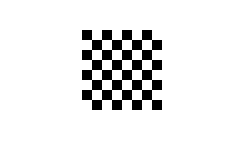
\includegraphics[width=\textwidth]{orig}
    \caption{Original}
    \label{fig:orig}
  \end{subfigure}
  \begin{subfigure}[b]{.16\textwidth}
    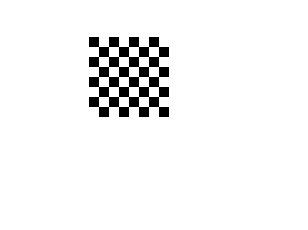
\includegraphics[width=\textwidth]{translate}
    \caption{Translate}
    \label{fig:trans}
  \end{subfigure}
  \begin{subfigure}[b]{.16\textwidth}
    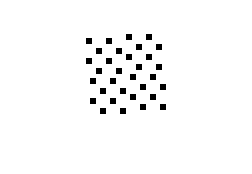
\includegraphics[width=\textwidth]{rotate}
    \caption{Rotate}
    \label{fig:rot}
  \end{subfigure}
  \begin{subfigure}[b]{.16\textwidth}
    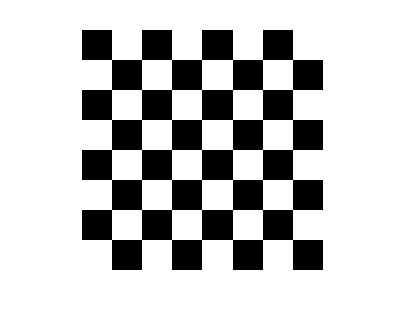
\includegraphics[width=\textwidth]{scale}
    \caption{Scale}
    \label{fig:scale}
  \end{subfigure}
  \begin{subfigure}[b]{.16\textwidth}
    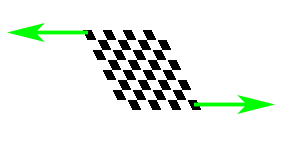
\includegraphics[width=\textwidth]{skew}
    \caption{Shear}
    \label{fig:skew}
  \end{subfigure}
  \begin{subfigure}[b]{.16\textwidth}
    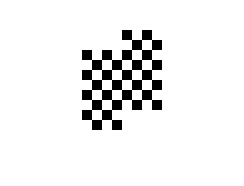
\includegraphics[width=\textwidth]{disjoint}
    \caption{Fracture}
    \label{fig:disj}
  \end{subfigure}
  \caption{Artificial dataset}
  \label{fig:artificial}
\end{figure}

Each of the above sequences was generated by the following affine transformation matrices respectively:

\begin{align*}
  \begin{bmatrix}
  1 & 0 & T_x \\
  0 & 1 & T_y \\
  0 & 0 & 1 \\
  \end{bmatrix}
  \hspace{1em}
  \begin{bmatrix}
  \cos(\theta) & -\sin(\theta) & 0 \\
  \sin(\theta) & \cos(\theta) & 0 \\
  0 & 0 & 1 \\
  \end{bmatrix}
  \hspace{1em}
  \begin{bmatrix}
  S_x & 0 & 0 \\
  0 & S_y & 0 \\
  0 & 0 & 1 \\
  \end{bmatrix}
  \hspace{1em}
  \begin{bmatrix}
  1 & 0 & 0 \\
  S & 1 & 0 \\
  0 & 0 & 1 \\
  \end{bmatrix}
\end{align*}

From left to right, the above transformation matrices represent: 
\begin{itemize}
  \item A translation, of $T_x$ pixels in the x-direction and $T_y$ pixels in the y direction
  \item A rotation of $\theta$ degrees about the centroid of the \verb|checkerboard| pattern
  \item A scaling of $S_x$ in the x-direction and $S_y$ in the y direction
  \item A shear parallel to the x-axis of S pixels i.e. $x' = x + ky$
\end{itemize}

The fracture is represented in MATLAB as two separate translations applied to two halves of the original \verb|checkerboard| pattern. For this dataset $T_x = -5i, T_y = -5i, \theta = 1^\circ, S_y = (i+1)/2, S_x = (i+1)/2$ and $S = 0.5$ where $i$ is the frame of the video being generated. The fracture had transformation equivalent to a translation with $T_y = sgn(y)2i$ applied to it, where the centroid of the \verb|checkerboard| pattern is coincident with the origin. Each transformation is applied repeatedly in order to generate sample sequences ten frames long. The MATLAB code used to generate the rotation sample sequence can be seen in code listing~\ref{lst:rotation}. The complete MATLAB code listing used to generate all the sample sequences can be seen in code listing~\ref{lst:generate} in Appendix~\ref{sec:appendix}.

\singlespacing
\begin{lstlisting}[language=MATLAB,caption={MATLAB code for creating rotation sample sequence},label=lst:rotation]
  theta=1;
  tform=affine2d([cosd(theta) -sind(theta) 0; sind(theta) cosd(theta) 0; 0 0 1]);
  writerObj = VideoWriter('rotate.avi');
  open(writerObj);
  frame=uint8(padarray(orig,[200 200],255).*255);
  writeVideo(writerObj,frame);
  r=imwarp(orig,tform,'FillValue',255);
  for i=1:10
    dr=size(r,1)-size(orig,1);
    dc=size(r,2)-size(orig,2);
    frame=uint8(padarray(r,[200-dr/2 200-dc/2],255).*255);
    writeVideo(writerObj,frame);
    r=imwarp(r,tform,'FillValue',255);
  end
  close(writerObj);
\end{lstlisting}
\onehalfspacing

In order to evaluate the algorithms more rigorously, the five sample sequences were sub sampled by $\frac{1}{2}, \frac{1}{4}, \frac{1}{8}$ and $\frac{1}{16}$ of the original size. In addition, as the Lucas-Kanade algorithm is a sparse optical flow algorithm, in order to make the comparison more rigorous when selecting points to track a set of all the pixels in the image was passed to the algorithm. This effectively makes the Lucas-Kanade algorithm a dense optical flow algorithm.

In order to measure the accuracy of the optical flow algorithm, as stated previously, it is required to know the optical flow that each of the transformations cause in the sample sequences. Therefore it was necessary to calculate the velocity field of each of the transformations as they were applied to the \verb|checkerboard| pattern. The MATLAB code written to calculate the velocity field for an arbitrary image which has an arbitrary transformation matrix applied to it can be seen in full in code listing~\ref{lst:velflow} in Appendix~\ref{sec:appendix}, however the key parts of the algorithm can be seen below, in code listing~\ref{lst:velfield}.

\singlespacing
\begin{lstlisting}[language=MATLAB,caption={MATLAB code to calculate the velocity field of a transformation matrix},label=lst:velfield]
% Set up matrix of points r0.
r0 = ones(n*m, 3);
n_ = -n/2;
m_ = -m/2;
for i = 1:n
  r0(i:m:(n*m),2) = n_;
  n_ = n_ + 1;
end
for j = 1:m
  r0((n*(j-1) + 1):n*j,1) = m_;
  m_ = m_ + 1;
end

% Calculate new positions for all points r0 after transformation under
%   tform, which are r1.
r1 = r0*tform.T;
r1(:,1) = r1(:,1)./r1(:,3);
r1(:,2) = r1(:,2)./r1(:,3);

% Eliminate third column (now unneeded)
r0_ = r0(:,1:2);
r1_ = r1(:,1:2);

% Calculate stacked matrix of velocities, v.
v = r1_ - r0_;

% Reshape v into V
V = reshape(v, [n m 2]);
r0 = reshape(r0_, [n m 2]);
r1 = reshape(r1_, [n m 2]);
\end{lstlisting}
\onehalfspacing

It should be noted that while we are only investigating individual affine transformations, the code listed in code listing~\ref{lst:velfield} and the full code in code listing~\ref{lst:velflow} in Appendix~\ref{sec:appendix} also work for arbitrary affine transformation matrices, in addition to projective transformation matrices.

Figure~\ref{fig:shearfield} shows the output from the velocity field calculation plotted using the MATLAB \verb|quiver| function. While at this scale it is impossible to discern the magnitude, or the direction to any degree of accuracy, it can be seen that the magnitude of the velocity grows in proportion to the absolute value of the y-coordinate. 

\begin{figure}[h]
  \centering
  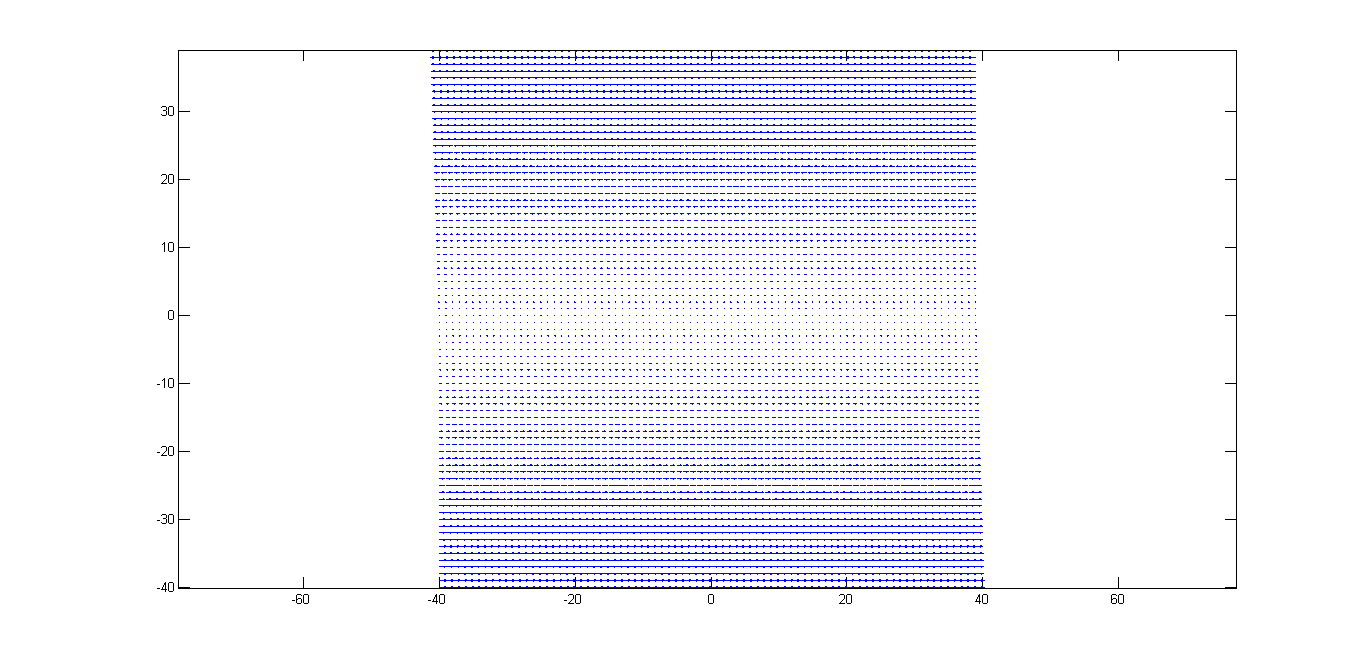
\includegraphics[width=\textwidth]{shear.png}
  \caption{Velocity field calculate for a shear}
  \label{fig:shearfield}
\end{figure}

\subsection{Real World Data}

In order to examine the algorithms in a real world scenario I was graciously provided with data sets from Dr Alexandre Kabla~\cite{harris2012characterizing}, a lecturer and researcher in CUED, and Mustafa Kamal, A PhD student in the Hopkinson Lab. Figure~\ref{fig:kamal} shows flow-flame interactions and comes from a high speed PIV dataset. Figure~\ref{fig:kabla} shows a cultured cell monolayer undergoing tensile testing.

\begin{figure}[htbp!]
  \centering
  \begin{subfigure}[b]{0.49\textwidth}
    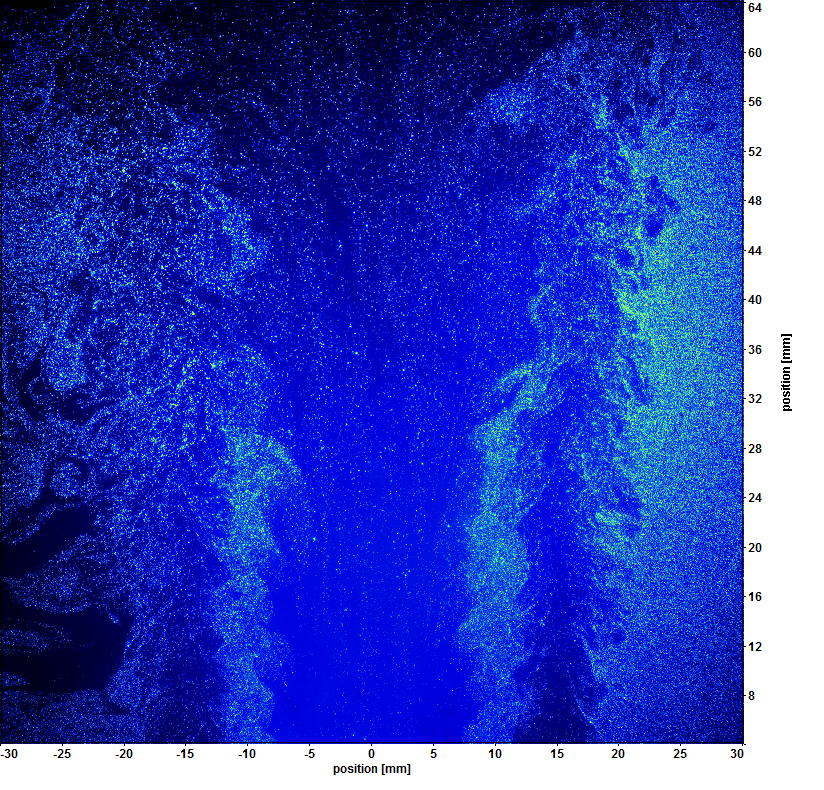
\includegraphics[width=\textwidth]{kamal}
    \caption{flow-flame interactions from a high speed PIV dataset}
    \label{fig:kamal}
  \end{subfigure}
  \begin{subfigure}[b]{0.49\textwidth}
    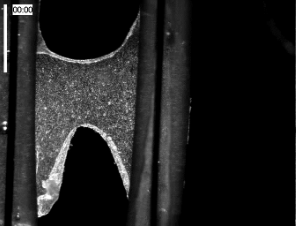
\includegraphics[width=\textwidth]{kabla}
    \caption{A cultured cell monolayer undergoing tensile testing}
    \label{fig:kabla}
  \end{subfigure}
  \caption{Real world data sets used}
  \label{fig:realworld}
\end{figure}

As there is no accurate, prior knowledge of the vector flow field, these datasets can only be used to compare the three optical flow algorithms for speed quantitatively, and for accuracy qualitatively. Also, for testing of real world data the Lucas-Kanade algorithm was used as a true sparse optical flow algorithm as opposed to its use in testing the artificial data where it was forced to track all pixels. It selected which pixels to track by calculating the minimal eigenvalue of gradient matrices for corner detection and selecting those pixels higher than a given threshold.